% Lezione del 21/04/2021

\documentclass[../main.tex]{subfiles}

\begin{document}
    \chapter{Modalità di indirizzamento}
    Qui di seguito sono elencati i modi di indirizzamento.
    \section{Register addressing (dato nel registro)}
    Operazioni che lavorano esclusivamente con registri
    \begin{itemize}
        \item \texttt{add \$s0, \$t2, \$t3}
        \item \texttt{sub \$t8, \$s1, \$0}
    \end{itemize}
    \section{Immediate addressing (dato nell'istruzione)}
    È possibile esprimere un operando attraverso un valore costante,
    che viene chiamato immediato ed occupa una parte del formato
    dell'istruzione (16 bit)
    \begin{itemize}
        \item \texttt{addi \$s4, \$t5, -73}
        \item \texttt{ori \$t3, \$t7, 0xFF}
    \end{itemize}
    \section{Base Addressing, ovvero attraverso una base (dato in memoria)}
    L'istruzione specifica l'indirizzo del dato, ovvero \\
    \texttt{indirizzo base + immediato con estensione del segno}
    \begin{itemize}
        \item \texttt{lw \$s4, 72(\$0) \hspace*{0cm} \hspace*{0cm}} \hspace*{1cm} \texttt{indirizzo = \$0 + 72}
        \item \texttt{sw \$t2, -25(\$t1)} \hspace*{1cm} \texttt{indirizzo = \$t1 - 25}
    \end{itemize}
    \section{PC-relative addressing}
    \begin{table}[h!]
        \begin{minipage}{.03\linewidth}
            \hspace*{0cm}
        \end{minipage}
        \begin{minipage}{.97\linewidth}
            \begin{tabular}{ l l l }
                \textbf{\texttt{0x10}} & & \texttt{beq \$t0, \$0, else} \\
                \textbf{\texttt{0x14}} & & \texttt{addi \$v0, \$0, 1} \\
                \textbf{\texttt{0x18}} & & \texttt{addi \$sp, \$sp, i} \\
                \textbf{\texttt{0x1C}} & & \texttt{jr \$ra} \\
                \textbf{\texttt{0x20}} & \texttt{else:} & \texttt{addi \$a0, \$a0, -1} \\
                \textbf{\texttt{0x24}} & & \texttt{jal factorial} \\
            \end{tabular}
        \end{minipage}
    \end{table}

    \noindent
    I 16 bit del campo immediato definiscono il numero di istruzioni
    tra la \textbf{branch target address} (\textbf{BTA}, ovvero
    l'indirizzo obiettivo del salto) e l'istruzione successiva
    al salto (l'istruzione nella posizione \texttt{PC + 4}).

    \begin{table}[h!]
        \begin{minipage}{.07\linewidth}
            \hspace*{0cm}
        \end{minipage}
        \begin{minipage}{.245\linewidth}
            \textbf{Codice MIPS assembly} \\
            \texttt{
                beq \$t0, \$0, else \\
                (beq \$t0, \$0, 3)
            }
        \end{minipage}
        \begin{minipage}{.675\linewidth}
            \caption*{\textbf{Valori dei campi}}
            \setlength{\tabcolsep}{0pt}

            \centering
            \begin{tabular}{ c | c | c | c | c | c }
                \vspace*{-4.2mm} & \multicolumn{1}{ p{(\linewidth / 48) * 6} }{} & \multicolumn{1}{ p{(\linewidth / 48) * 5} }{} & \multicolumn{1}{ p{(\linewidth / 48) * 5} }{} & \multicolumn{1}{ p{(\linewidth / 48) * 16} }{} \\
                \\[-9mm]
                \multicolumn{1}{ c }{\multirow{2}{*}{}} &
                \multicolumn{1}{ c }{\multirow{2}{*}{op}} &
                \multicolumn{1}{ c }{\multirow{2}{*}{rs}} &
                \multicolumn{1}{ c }{\multirow{2}{*}{rt}} &
                \multicolumn{1}{ c }{\multirow{2}{*}{imm}} &
                \\[-4.4mm]
                & & & & \\[2.4mm]
                \cline{2-5}
                \multicolumn{1}{ c | }{} & 4 & 8 & 0 & 3 & \\
                \cline{2-5}
                \multicolumn{1}{ c }{\rule{0pt}{.8\normalbaselineskip}} & \multicolumn{1}{ c }{6 bits} & \multicolumn{1}{ c }{5 bits} & \multicolumn{1}{ c }{5 bits} & \multicolumn{1}{ c }{16 bits} & \\
            \end{tabular}
        \end{minipage}
    \end{table}

    \begin{table}[h!]
        \begin{minipage}{.03\linewidth}
            \hspace*{0cm}
        \end{minipage}
        \begin{minipage}{.97\linewidth}
            \subsection*{Esercizio}
            Calcolare il campo immediato per l'istruzione \texttt{bne}
            (che valore viene messo nel campo {\color{blue} \textbf{loop}}?).
        \end{minipage}

        \vspace*{3mm}

        \begin{minipage}{.06\linewidth}
            \hspace*{0cm}
        \end{minipage}
        \begin{minipage}{.94\linewidth}
            \begin{tabular}{ l l l }
                \textbf{\texttt{0x40}} & \texttt{{\color{blue} \textbf{loop}}:} & \texttt{add \hspace*{0cm} \hspace*{0cm} \$t1, \$a0, \$s0} \\
                \textbf{\texttt{0x44}} & & \texttt{lb \hspace*{0cm} \hspace*{0cm} \hspace*{0cm} \$t1, 0(\$t1)} \\
                \textbf{\texttt{0x48}} & & \texttt{add \hspace*{0cm} \hspace*{0cm} \$t2, \$a1, \$s0} \\
                \textbf{\texttt{0x4C}} & & \texttt{sb \hspace*{0cm} \hspace*{0cm} \hspace*{0cm} \$t1, 0(\$t2)} \\
                \textbf{\texttt{0x50}} & & \texttt{addi \hspace*{0cm} \$s0, \$s0, 1} \\
                \textbf{\texttt{0x54}} & & \texttt{bne \hspace*{0cm} \hspace*{0cm} \$t1, \$0, {\color{blue} \textbf{loop}}} \\
                \textbf{\texttt{0x58}} & & \texttt{lw \hspace*{0cm} \hspace*{0cm} \hspace*{0cm} \$s0, 0(\$sp)} \\
            \end{tabular}
        \end{minipage}

        \vspace*{3mm}

        \begin{minipage}{.03\linewidth}
            \hspace*{0cm}
        \end{minipage}
        \begin{minipage}{.94\linewidth}
            \underline{\textbf{Risposta}: il campo {\color{blue} \textbf{loop}} vale \texttt{-6}.}
        \end{minipage}
    \end{table}

    \newpage

    \section{Pseudo-direct addressing}

    \begin{table}[h!]
        \begin{minipage}{.03\linewidth}
            \hspace*{0cm}
        \end{minipage}
        \begin{minipage}{.97\linewidth}
            \begin{tabular}{ l l l }
                \textbf{\texttt{0x0040005C}} & & \texttt{jal sum} \\
                \textbf{\texttt{\dots}} & & \\
                \textbf{\texttt{0x004000A0}} & \texttt{sum:} & \texttt{add \$v0, \$a0, \$a1} \\
            \end{tabular}
        \end{minipage}
    \end{table}

    \noindent
    Il processore calcola il \textbf{jump target address}
    (\textbf{JTA}, ovvero l’indirizzo obiettivo del salto)
    dall'istruzione di tipo J aggiungendo 2 zeri alla fine
    e sostituendo le prime 4 cifre con i 4 bit più significativi
    dell'indirizzo \texttt{PC + 4} al campo dell'indirizzo da 26 bit.
    
    \begin{table}[h!]
        \renewcommand{\arraystretch}{1.25}
        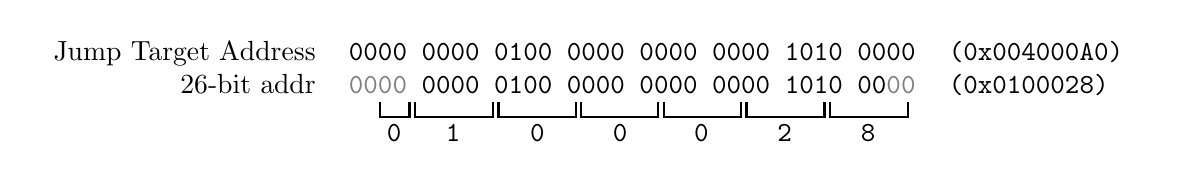
\begin{tikzpicture}
            \node(table) {
                \begin{tabular}{ r c l }
                    Jump Target Address & \texttt{0000 0000 0100 0000 0000 0000 1010 0000} & \texttt{(0x004000A0)} \\
                    26-bit addr & \texttt{{\color{gray}0000} 0000 0100 0000 0000 0000 1010 00{\color{gray}00}} & \texttt{(0x0100028)} \\
                \end{tabular}
            };

            \draw [thick]
                (-2.65,-.4) -- (-2.65,-.6) -- (-2.27,-.6) -- (-2.27,-.4);
            \node [text width=1.75mm] at (-2.47,-.8) {\texttt{0}};

            \draw [thick]
                (-2.2,-.4) -- (-2.2,-.6) -- (-1.21,-.6) -- (-1.21,-.4);
            \node [text width=1.75mm] at (-1.72,-.8) {\texttt{1}};

            \draw [thick]
                (-1.14,-.4) -- (-1.14,-.6) -- (-.16,-.6) -- (-.16,-.4);
            \node [text width=1.75mm] at (-.65,-.8) {\texttt{0}};

            \draw [thick]
                (-.09,-.4) -- (-.09,-.6) -- (.89,-.6) -- (.89,-.4);
            \node [text width=1.75mm] at (.4,-.8) {\texttt{0}};

            \draw [thick]
                (.96,-.4) -- (.96,-.6) -- (1.94,-.6) -- (1.94,-.4);
            \node [text width=1.75mm] at (1.43,-.8) {\texttt{0}};

            \draw [thick]
                (2.01,-.4) -- (2.01,-.6) -- (3,-.6) -- (3,-.4);
            \node [text width=1.75mm] at (2.49,-.8) {\texttt{2}};

            \draw [thick]
                (3.07,-.4) -- (3.07,-.6) -- (4.06,-.6) -- (4.06,-.4);
            \node [text width=1.75mm] at (3.55,-.8) {\texttt{8}};
        \end{tikzpicture}
    \end{table}

    \begin{table}[h!]
        \begin{minipage}{.07\linewidth}
            \hspace*{0cm}
        \end{minipage}
        \begin{minipage}{.245\linewidth}
            \caption*{\textbf{Valori dei campi}}
            \setlength{\tabcolsep}{6pt}

            \centering
            \begin{tabular}{ c | c | c | c }
                \vspace*{-4.2mm} & \multicolumn{1}{ p{(\linewidth / 48) * 6} }{} & \multicolumn{1}{ p{(\linewidth / 48) * 26} }{} \\
                \\[-9mm]
                \multicolumn{1}{ c }{\multirow{2}{*}{}} &
                \multicolumn{1}{ c }{\multirow{2}{*}{op}} &
                \multicolumn{1}{ c }{\multirow{2}{*}{imm}} &
                \\[-4.4mm]
                & & \\[2.4mm]
                \cline{2-3}
                \multicolumn{1}{ c | }{} & \texttt{3} & \texttt{0x0100028} & \\
                \cline{2-3}
                \multicolumn{1}{ c }{\rule{0pt}{.8\normalbaselineskip}} & \multicolumn{1}{ c }{6 bits} & \multicolumn{1}{ c }{26 bits} & \\
            \end{tabular}
        \end{minipage}
        \begin{minipage}{.675\linewidth}
            \caption*{\textbf{Codice macchina}}
            \setlength{\tabcolsep}{6pt}

            \centering
            \begin{tabular}{ c | c | c | c }
                \vspace*{-4.2mm} & \multicolumn{1}{ p{(\linewidth / 48) * 6} }{} & \multicolumn{1}{ p{(\linewidth / 48) * 26} }{} \\
                \\[-9mm]
                \multicolumn{1}{ c }{\multirow{2}{*}{}} &
                \multicolumn{1}{ c }{\multirow{2}{*}{op}} &
                \multicolumn{1}{ c }{\multirow{2}{*}{imm}} &
                \\[-4.4mm]
                & & \\[2.4mm]
                \cline{2-3}
                \multicolumn{1}{ c | }{} & \texttt{000011} & \texttt{00 0001 0000 0000 0000 0010 1000} & \\
                \cline{2-3}
                \multicolumn{1}{ c }{\rule{0pt}{.8\normalbaselineskip}} & \multicolumn{1}{ c }{6 bits} & \multicolumn{1}{ c }{26 bits} & \\
            \end{tabular}
        \end{minipage}
    \end{table}

    \noindent
    \underline{\textbf{Nota bene}: Poiché i 4 bit più sigificativi
    sono presi da \texttt{PC + 4} il range del salto è limitato.}

    \section{Modello riassuntivo}
    \begin{table}[h!]
        \setlength{\tabcolsep}{0pt}
        \renewcommand{\arraystretch}{2}

        \underline{Operando - \textbf{Register addressing}} \\[-2mm]
        \begin{tikzpicture}
            \node(table) {
                \begin{tabular}{ c c | c | c | c | c | c | c | c | }
                    \vspace*{-4.2mm} & \multicolumn{1}{ p{(\linewidth / 64) * 6} }{} & \multicolumn{1}{ p{(\linewidth / 64) * 5} }{} & \multicolumn{1}{ p{(\linewidth / 64) * 5} }{} & \multicolumn{1}{ p{(\linewidth / 64) * 5} }{} & \multicolumn{1}{ p{(\linewidth / 64) * 5} }{} & \multicolumn{1}{ p{(\linewidth / 64) * 6} }{} & \multicolumn{1}{ p{(\linewidth / 64) * 8} }{} & \multicolumn{1}{ p{(\linewidth / 64) * 24} }{} \\
                    \cline{2-7}
                    \multicolumn{1}{ c | }{} & \texttt{op} & \texttt{rs} & \texttt{rt} & \texttt{rd} & \texttt{shamt} & \texttt{funct} & \multicolumn{1}{ c }{} & \multicolumn{1}{ c }{Register} \\
                    \cline{2-7}
                    \cline{9-9}
                    \multicolumn{1}{ c }{} & \multicolumn{1}{ c }{} & \multicolumn{1}{ c }{} & \multicolumn{1}{ c }{} & \multicolumn{1}{ c }{} & \multicolumn{1}{ c }{} & \multicolumn{1}{ c }{} & \multicolumn{1}{ c | }{} & word operand \\
                    \cline{9-9}
                \end{tabular}
            };

            \draw [->, thick]
                (-6.06,-.22) -- (-6.06,-.62) -- (2.06,-.62);

        \end{tikzpicture}

        \vspace*{1mm}

        \underline{Operando - \textbf{Immediate addressing}} \\[-2mm]
        \begin{tabular}{ c c | c | c | c | c }
            \vspace*{-4.2mm} & \multicolumn{1}{ p{(\linewidth / 64) * 6} }{} & \multicolumn{1}{ p{(\linewidth / 64) * 5} }{} & \multicolumn{1}{ p{(\linewidth / 64) * 5} }{} & \multicolumn{1}{ p{(\linewidth / 64) * 16} }{} \\
            \cline{2-5}
            \multicolumn{1}{ c | }{} & \texttt{op} & \texttt{rs} & \texttt{rt} & \texttt{imm} & \\
            \cline{2-5}
        \end{tabular}

        \vspace*{8mm}

        \underline{Operando - \textbf{Base addressing}} \\[-2mm]
        \begin{tikzpicture}
            \node(table) {
                \begin{tabular}{ c c | c | c | c | c | c | }
                    \vspace*{-4.2mm} & \multicolumn{1}{ p{(\linewidth / 64) * 6} }{} & \multicolumn{1}{ p{(\linewidth / 64) * 5} }{} & \multicolumn{1}{ p{(\linewidth / 64) * 5} }{} & \multicolumn{1}{ p{(\linewidth / 64) * 16} }{} & \multicolumn{1}{ p{(\linewidth / 64) * 8} }{} & \multicolumn{1}{ p{(\linewidth / 64) * 24} }{} \\
                    \cline{2-5}
                    \multicolumn{1}{ c | }{} & \texttt{op} & \texttt{rs} & \texttt{rt} & \texttt{offset} & \multicolumn{1}{ c }{} & \multicolumn{1}{ c }{Memory} \\
                    \cline{2-5}
                    \cline{7-7}
                    \multicolumn{1}{ c }{} & \multicolumn{1}{ c }{} & \multicolumn{1}{ c }{} & \multicolumn{1}{ c }{} & \multicolumn{1}{ c }{} & \multicolumn{1}{ c | }{} & word or byte operand \\
                    \cline{7-7}
                    \cline{1-5}
                    \multicolumn{5}{ | c | }{base register} \\
                    \cline{1-5}
                \end{tabular}
            };

            \draw [->, thick]
                (-6.06,.2) -- (-6.06,-.64);

            \draw [->, thick]
                (-2.05,.2) -- (-2.05,0) -- (.2,0) -- (.2,.41) -- (.68,.41);

            \draw [->, thick]
                (-4.13,-.64) -- (-4.13,-.44) -- (.2,-.44) -- (.2,-.85) -- (.68,-.85);

            \draw (1,-.22) node[one bit adder,scale=.75]{\Large \textbf{+}};

            \draw [->, thick]
                (1.32,-.22) -- (2.06,-.22);
            
            \draw [-, white, thick]
                (1,-.87) -- (1,-1.07);

        \end{tikzpicture}

        \vspace*{5mm}

        \underline{Istruzione - \textbf{PC-relative addressing}} \\[-2mm]
        \begin{tikzpicture}
            \node(table) {
                \begin{tabular}{ c c | c | c | c | c | c | }
                    \vspace*{-4.2mm} & \multicolumn{1}{ p{(\linewidth / 64) * 6} }{} & \multicolumn{1}{ p{(\linewidth / 64) * 5} }{} & \multicolumn{1}{ p{(\linewidth / 64) * 5} }{} & \multicolumn{1}{ p{(\linewidth / 64) * 16} }{} & \multicolumn{1}{ p{(\linewidth / 64) * 8} }{} & \multicolumn{1}{ p{(\linewidth / 64) * 24} }{} \\
                    \cline{2-5}
                    \multicolumn{1}{ c | }{} & \texttt{op} & \texttt{rs} & \texttt{rt} & \texttt{offset} & \multicolumn{1}{ c }{} & \multicolumn{1}{ c }{Memory} \\
                    \cline{2-5}
                    \cline{7-7}
                    \multicolumn{1}{ c }{} & \multicolumn{1}{ c }{} & \multicolumn{1}{ c }{} & \multicolumn{1}{ c }{} & \multicolumn{1}{ c }{} & \multicolumn{1}{ c | }{} & branch destination instruction \\
                    \cline{7-7}
                    \cline{1-5}
                    \multicolumn{5}{ | c | }{Program Counter (PC)} \\
                    \cline{1-5}
                \end{tabular}
            };

            \draw [->, thick]
                (-2.05,.2) -- (-2.05,0) -- (.2,0) -- (.2,.41) -- (.68,.41);

            \draw [->, thick]
                (-4.13,-.64) -- (-4.13,-.44) -- (.2,-.44) -- (.2,-.85) -- (.68,-.85);

            \draw (1,-.22) node[one bit adder,scale=.75]{\Large \textbf{+}};

            \draw [->, thick]
                (1.32,-.22) -- (2.06,-.22);
            
            \draw [-, white, thick]
                (1,-.87) -- (1,-1.07);

        \end{tikzpicture}

        \vspace*{5mm}

        \underline{Istruzione - \textbf{Pseudo-direct addressing}} \\[-2mm]
        \begin{tikzpicture}
            \node(table) {
                \begin{tabular}{ c c | c | c | c | }
                    \vspace*{-4.2mm} & \multicolumn{1}{ p{(\linewidth / 64) * 6} }{} & \multicolumn{1}{ p{((\linewidth / 64) * 26)} }{} & \multicolumn{1}{ p{(\linewidth / 64) * 8} }{} & \multicolumn{1}{ p{(\linewidth / 64) * 24} }{} \\
                    \cline{2-3}
                    \multicolumn{1}{ c | }{} & \texttt{op} & \texttt{jump address} & \multicolumn{1}{ c }{} & \multicolumn{1}{ c }{Memory} \\
                    \cline{2-3}
                    \cline{5-5}
                    \multicolumn{1}{ c }{} & \multicolumn{1}{ c }{} & \multicolumn{1}{ c }{} & \multicolumn{1}{ c | }{} & jump destination instruction \\
                    \cline{5-5}
                    \cline{1-3}
                    & \multicolumn{1}{ | c }{ \cellcolor{black} \color{white} \textbf{\texttt{4 bit\hspace*{0cm} }} } & \multicolumn{1}{ | c | }{Program Counter (PC)} \\
                    \cline{1-3}
                \end{tabular}
            };

            \draw [->, thick]
                (-3.35,.2) -- (-3.35,0) -- (.2,0) -- (.2,.41) -- (.68,.41);

            \draw [->, thick]
                (-7.5,-.64) -- (-7.5,-.44) -- (.2,-.44) -- (.2,-.85) -- (.68,-.85);

            \draw (.96,-.22) ellipse (3.6mm and 1cm);
            \node [text width=3.6mm] at (.96,-.22) {\Large \textbf{\hspace*{.5mm}$\parallel$}};

            \draw [->, thick]
                (1.32,-.22) -- (2.06,-.22);
            
            \draw [-, white, thick]
                (1,-.87) -- (1,-1.07);

        \end{tikzpicture}
    \end{table}
\end{document}